\section{Peuplement semi-automatique d'ontologies métiers}

Bien que Word2Vec fournisse des termes similaires pertinents, du bruit est toujours présent. Aussi il n'est possible pour l'heure d'automatiser complètement le processus. Nous avons donc développé une application web, Curiositext, permettant à un utilisateur non expert de visualiser les résultats de Word2Vec et de peupler semi-automatiquement une ontologie métier. Celle-ci est indépendante de l'architecture de l'application qui s'adapte par conséquent au cas d'usage étudié, sans dépendance à un domaine spécifique. Dans un premier temps, l'utilisateur est invité à charger un corpus texte local ou peut effectuer une requête à l'aide d'Elasticsearch \footnote{www.elastic.co} pour récupérer des données distantes. Il peut ensuite appliquer Word2Vec sur ses données. Les paramètres de base de la méthode sont paramétrables à savoir : la dimension des vecteurs, la taille de la fenêtre, la fréquence minimale d'apparition d’un terme pour l’apprentissage, le modèle (CBOW ou Skip-Gram) et le nombre d’itérations.
%
\begin{figure}[tb]
    \begin{center}
        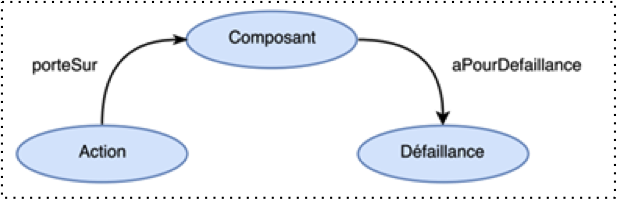
\includegraphics[width=9cm]{figures/ontMetier}
    \end{center}
    \caption{Ontologie métier}\label{fig:metier}
\end{figure}
%
L'utilisateur accède ensuite à la troisième partie de l'application à savoir le peuplement d'une ontologie. Il doit charger l’ontologie métier qu'il souhaite peupler et qu'il a modélisée en amont (fig \ref{fig:metier}). Pour ce faire, nous avons mis en place un scénario de peuplement de l'ontologie finale illustré ici par la requête du terme \texttt{changement}.
Pour aider au peuplement de l'ontologie, une ontologie linguistique (fig \ref{fig:ling}) a été intégrée dans l'application. L'utilisateur doit renseigner pour le terme requêté sa classe lexicale (\texttt{Terme\_Canonique}) et sa classe métier (ici \texttt{Action}).
%
\begin{figure}[tb]
    \begin{center}
        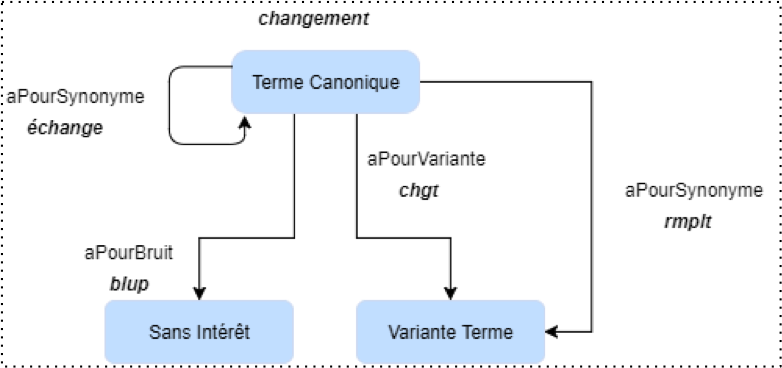
\includegraphics[width=9cm]{figures/ontLing}
    \end{center}
    \caption{Ontologie linguistique}\label{fig:ling}
\end{figure}
%
Grâce à l'utilisation d'un entrepôt RDF comme backend de l'application, nous bénéficions, outre les capacités de requêtage et de stockage, des possibilités de raisonnement définies lors de la création des ontologies. Ainsi, l'interface ne fournit que les informations essentielles issues des déductions effectuées par l'entrepôt ; il se charge de les compléter à l'aide de la formalisation OWL (RL)\cite{owlprofiles} définie dans les ontologies. Par exemple, le fait d'ajouter un lien de synonymie ou de variance dans les données permet le cas échéant de déduire l'appartenance d'un individu à une classe métier (ici \texttt{Action}) grâce à l'axiome ci-dessous\footnote{Notons que nous sommes obligés de dupliquer ce type d'axiome pour chaque classe concernée.
} :
$$
\begin{array}{ll}
\exists  \ \texttt{aPourSynonyme} .  \texttt {Action}  \sqcup \exists  \ \texttt{aPourVariante} .  \texttt {Action}
\sqsubseteq    \texttt{Action}
\end{array}
$$
En logique de description, cela signifie que tout individu qui a un synonyme ou une variante dans la classe \texttt{Action} appartient à la classe \texttt{Action} lui-même. Nous faisons la même chose pour les classes \texttt{Composant} et \texttt{Defaillance}, la logique du premier ordre ne nous permettant pas d'écrire des axiomes sur des ensembles de classes.
L'interface ne fait qu'ajouter ou retirer des triplets RDF élémentaires, l'intelligence de l'entrepôt se charge de faire les mises à jour déclenchées par le raisonnement et éventuellement de détecter des incohérences dans les données.
